\chapter{IoT Design Aspects}
Each device is usually low power and low cost small and autonomous system, equipped with processor, memory and radio transceiver along with sensing and/or actuating elements, with everything being powered a battery (or something equivalent such as solar cells).

The main limitations in the design of IoT devices are due to the abovementioned components ---aside from the sensors/actuators--- and is not clear whether technology improvements will overcome such constraints.  

\section{Issues}
\begin{enumerate}
   \item Energy efficiency
   \begin{enumerate}
      \item sensors are battery-powered or use energy
      harvesting
      \item need for HW/SW energy efficient solutions
   \end{enumerate}
   \item Adaptatability to changing conditions
   \begin{enumerate}
      \item need for dynamic network management and programming
   \end{enumerate}
   \item Low-complexity, low overhead protocols
   \begin{enumerate}
      \item need at any level of the protocol stack due
      to limitation of nodes’ resources
   \end{enumerate}
   \item Security
   \begin{enumerate}
      \item at all layers ot the stack
   \end{enumerate}
   \item Multihop communications
   \begin{enumerate}
      \item need for protocol stacks and routing
      protocols
   \end{enumerate}
   \item Mobility
   \begin{enumerate}
      \item Need for dynamic routing protocols
      Data storage and (pre-)processing
   \end{enumerate}
\end{enumerate}

\subsection{Moore's law}
\begin{center}
   
   \textit{``The number of transistors that can be (inexpensively) embedded in a chip grows exponentially''}
   
   In other words, \textit{``it doubles every two years''}
\end{center}

Three different ---but equally true--- interpretations may be given to such law:
\begin{enumerate}
   \item The performance doubles every two years at the same cost
   \note{Up to now this is true for processors of servers/desktops}
   \item The chip’s size halves every two years at the same cost
   \note{Consequently also the energy consumption is reduced}
   \item The size and the processing power remain the same but the cost
   halves every two years
\end{enumerate}

\section{Battery consumption}

\begin{figure}[htbp]
   \centering
   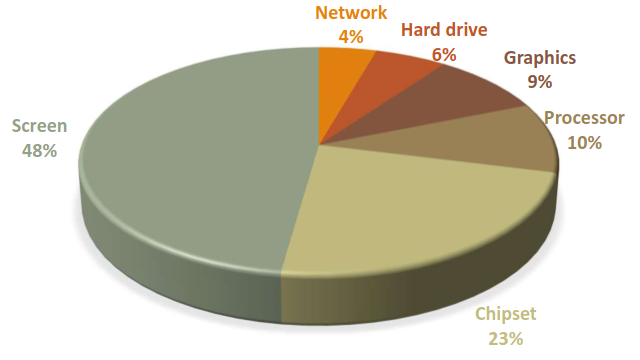
\includegraphics[width=0.45\columnwidth]{images/iot_laptop_consumption.png}
   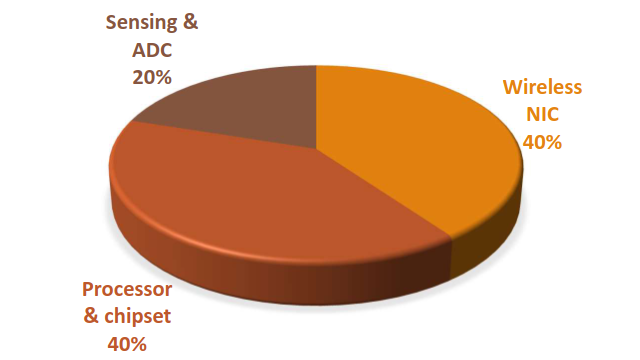
\includegraphics[width=0.45\columnwidth]{images/iot_sensor_consumption.png}
   \caption{Laptop and IoT Sensor battery consumption percentages}
   \label{fig:iot_sensor_consumption}
\end{figure}

In the previous decades the focus was on minimizing the number of bytes sent to optimize network performance.
For IoT instead, the focus is to \ul{keep the radio off most of the time}, since it consumes about 40\% of the battery.

\subsection{Duty Cycle}
Also turning off CPU and radio is battery consuming, so it must be done according to some criteria.\\
Since the activity of an IoT device is (mostly) repetitive, it may define a \textbf{duty cycle} by alternating periods of activity to periods of inactivity.
\begin{paracol}{2}
   
   The duty cycle of a system (or a component / device) is defined as the fraction of one period in which the system is active.
   \note{100\% means always active, while 1\% means active only 1\% of its period}

   Note that even if the duty cycle of the whole device may be defined at application level, \ul{each component has its own duty cycle}, adding some "unpredictability" to the power consumption equation. 
   \switchcolumn

   \begin{lstlisting}[language=C,otherkeywords = {turnOn,turnOff,idle,Serial}]
void loop() {
   // reads the input from analog pin 0:
   turnOn(analogSensor);
   int sensorValue = analogRead(A0);
   turnOff(analogSensor);
   // converts value into a voltage (0-5V):
   float voltage = sensorValue * (5.0 / 1023.0);
   // transmits voltage over the radio
   turnOn(radioInterface);
   Serial.println(voltage);
   turnOff(radioInterface);
   // waits for next loop
   idle(380);
}
   \end{lstlisting}
   
\end{paracol}


Sometimes the specification of an IoT device indicates the power consumption expressed in $mA$ for each component in each state it may be (idle/read/write/etc.).
Even if not completely precise, the specification may provide a good approximation of the consumption.\\
It is also important to note that there should be a record in the specs indicating how much capacity the battery loses over time. Most batteries lose a low percentage (e.g. 3\%) capacity each year.

\begin{figure}[htbp]
   \centering
   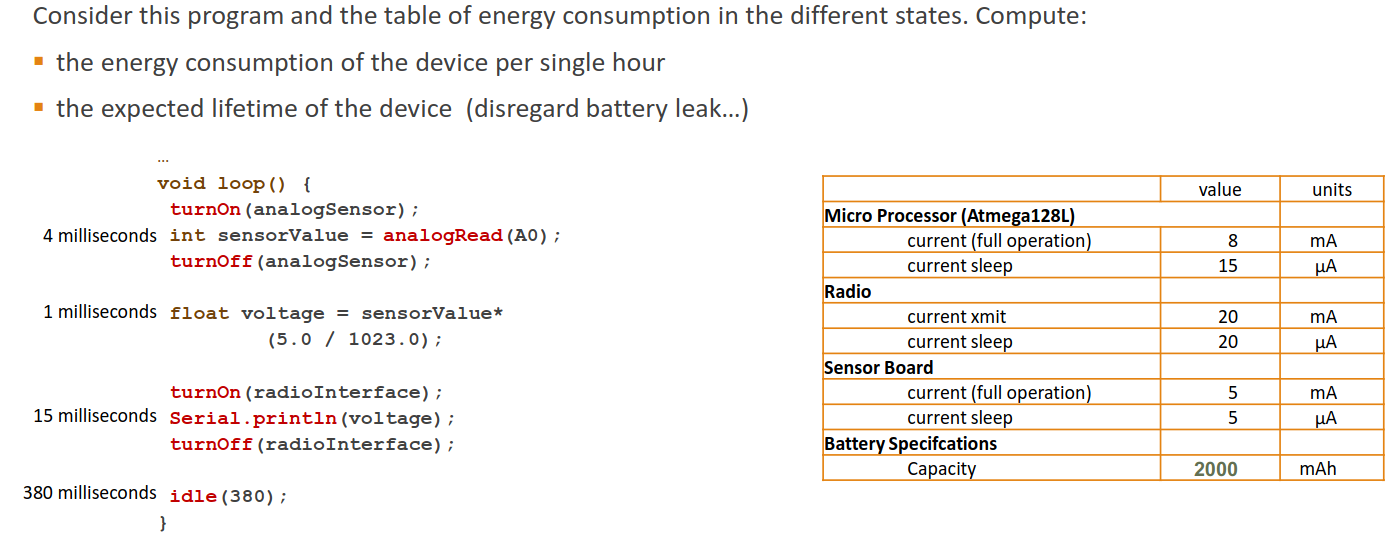
\includegraphics{images/energy_exercise.png}
   \caption{Exercise on energy consumption and duty cycling}
   \label{fig:energy_exercise}
\end{figure}
For what concerns the exercise, these are the calculations
\begin{table}[htbp]
   \centering
   \begin{tabular}{|c|c|c|c|c|}
      CPU & 5 &				0.05 * 8 	& 0.95 * 0.015	&	 0.41425\\
      Radio & 3,75 &		0.0375 * 20 	& 0.9625 * 0.020 &	 0.9425\\
      Sensor & 1 &			0.01 * 5		& 	0.99 * 0.005	&	 0.05495\\
   \end{tabular}
   \caption{Exercise calculations and solutions}
   \label{tab:battery_consumption}
\end{table}

\subsection{MAC Protocols}
In general they are Low-level communication protocols to send/receive packets to/from in-range sensors, but in IoT  they also implement strategies for energy efficiency, by synchronize devices and turning off the radio when it is not needed\footnote{Equivalent to excluding a device from the network}.

\subsection*{Exercise 1}
% Sampling time = 0.5ms * 5 = 2.5ms\\
% Periodo = 1/20 = 0.05s = 50ms\\
% Inactive time = 50ms*4 - 0.5ms * 4 = 198ms\\
% Energy sleeping = 198ms * (15 + 5)uA + (20uA)*200ms = 0.00792mA\\
% Energy active = 0.5ms * (8 + 5)mA = 6.5mA
% \nl

% Transmit time = 2ms * 5 = 10ms\\
% Energy sleeping = already computed\\
% Energy active = 10ms * (8 + 20)mA = 280mA
% \nl

% Total energy = 0.00792 + 6.5 + 0.00792 + 280 = 286.51592mA\\
% Total energy available = 2000mAh\\
% Expected lifetime = 2000 / 286.51592 = 6.98 hours

\begin{figure}[htbp]
   \centering
   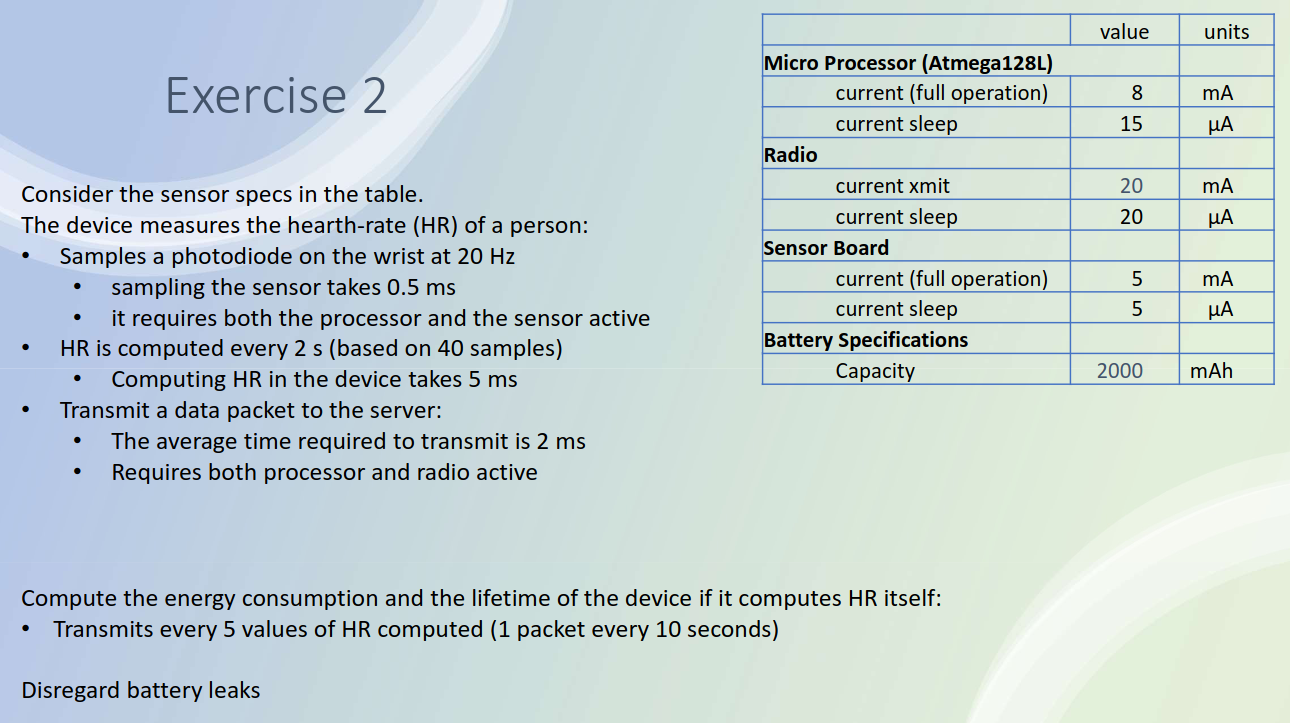
\includegraphics{images/energy_exercise1.png}
   \label{fig:energy_exercise1}
\end{figure}

Duty cycle sensor = 0.01\\
Duty cycle radio = 0.008\\
Duty cycle CPU = $(0.5 * 5 + 2)/250ms = 0.018 = 0.01 + 0.008$
\nl
\begin{align*}
   &\textbf{Radio energy} \texttt{ON} &=& 20mA * 0.008 &= 0.16mA\\ 
   &\textbf{Radio energy} \texttt{IDLE} &=& 20\mu A *0.992 &= 0.01984mA\\
   &\textbf{Sensor energy} \texttt{ON} &=& 5mA *0.01 &= 0.05mA\\
   &\textbf{Sensor energy} \texttt{IDLE} &=& 5\mu A *0.99 &= 0.00495mA\\
   &\textbf{CPU energy} \texttt{ON} &=& 8mA * 0.018 &= 0.144mA\\
   &\textbf{CPU energy} \texttt{IDLE} &=& 15\mu A * 0.982 &= 0.0147mA
\end{align*}

\textbf{Total energy} per hour =\\
$0.16 + 0.01984 + 0.05 + 0.00495 + 0.144 + 0.0147 = 0.39349mA$\\
Total energy available = 2000mAh\\
Expected lifetime = $2000 / 0.39349 = 5084.5h = 212d$

\subsection*{Exercise 2}
\begin{figure}[htbp]
   \centering
   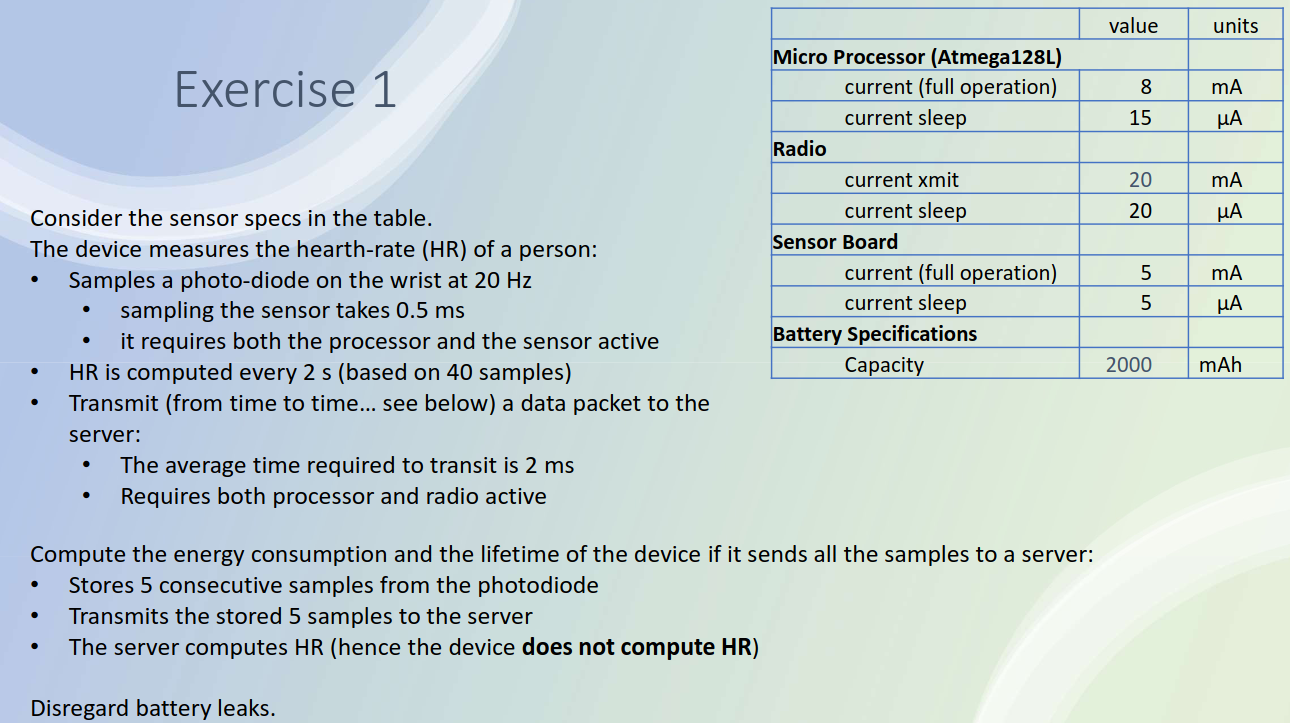
\includegraphics{images/energy_exercise2.png}
   \label{fig:energy_exercise2}
\end{figure}

Duty cycle sensor = 0.01\\
Duty cycle radio = $2 / 10000ms = 0.0002$\\
Duty cycle processor = $(0.5 * 200 + 2 + 5*5)/10000 = 0.0127$
\begin{align*}
   &\textbf{Radio energy} \texttt{ON} &=& 20mA * 0.0002 &= 0.004mA\\ 
   &\textbf{Radio energy} \texttt{IDLE} &=& 20\mu A * 0.9998 &= 0.01998mA\\
   &\textbf{Sensor energy} \texttt{ON} &=& 5mA *0.01 &= 0.05mA\\
   &\textbf{Sensor energy} \texttt{IDLE} &=& 5\mu A *0.99 &= 0.00495mA\\
   &\textbf{CPU energy} \texttt{ON} &=& 8mA * 0.0127 &= 0.1016mA\\
   &\textbf{CPU energy} \texttt{IDLE} &=& 15\mu A * 0.9873 &= 0.0148mA
\end{align*}

\textbf{Total energy} per hour =\\
$0.004 + 0.01998 + 0.05 + 0.00495 + 0.1016 + 0.0148 = 0.19533mA$\\
Total energy available = 2000mAh\\
Expected lifetime = $2000 / 0.19533 = 10238.5h = 426d$
